\chapter{行列 - Matrices}

\index{行列 - matrix}

\key{行列(matrix)} は、プログラミングにおける2次元配列に相当する数学の用語です。
\[
A =
 \begin{bmatrix}
  6 & 13 & 7 & 4 \\
  7 & 0 & 8 & 2 \\
  9 & 5 & 4 & 18 \\
 \end{bmatrix}
\]
はサイズ$3 \times 4$の行列であり、3行4列の行列と呼ばれます。
$[i, j]$という表記がよく用いられ、行列の$i$行$j$列を意味します。
例えば、上の行列では、$A[2,3]=8$ and $A[3,1]=9$です。
行列の特殊な例として、大きさが1次元の行列である\key{ベクトル}があります
つまり、$n \times 1$の行列のことで以下の様になります。
\index{ベクトル - vector}

\[
V =
\begin{bmatrix}
4 \\
7 \\
5 \\
\end{bmatrix}
\]

これは3つの要素からなるベクトルです。

\index{転置行列 - transpose}

\key{転置行列 - transpose} $A^T$ は $A$の行と列が入れ替わったものです。
つまり、$A^T[i,j]=A[j,i]$になります。例をみてみましょう。
\[
A^T =
 \begin{bmatrix}
  6 & 7 & 9 \\
  13 & 0 & 5 \\
  7 & 8 & 4 \\
  4 & 2 & 18 \\
 \end{bmatrix}
\]

\index{正方行列 - square matrix}

\key{正方行列 - square matrix}行と列が同じ数の行列は
正方行列と呼ばれます。例を示します。

\[
S =
 \begin{bmatrix}
  3 & 12 & 4  \\
  5 & 9 & 15  \\
  0 & 2 & 4 \\
 \end{bmatrix}
\]

\section{行列の演算 - Operations}

行列$A$と$B$の和$A+B$は、
行列が同じ大きさである場合に操作できます。
$A$と$B$の同じ行と列の要素の和が答えとなります。

\[
 \begin{bmatrix}
  6 & 1 & 4 \\
  3 & 9 & 2 \\
 \end{bmatrix}
+
 \begin{bmatrix}
  4 & 9 & 3 \\
  8 & 1 & 3 \\
 \end{bmatrix}
=
 \begin{bmatrix}
  6+4 & 1+9 & 4+3 \\
  3+8 & 9+1 & 2+3 \\
 \end{bmatrix}
=
 \begin{bmatrix}
  10 & 10 & 7 \\
  11 & 10 & 5 \\
 \end{bmatrix}.
\]

行列$A$に対する$x$での乗算は
各要素に$x$をかけたものとなります。
\[
 2 \cdot \begin{bmatrix}
  6 & 1 & 4 \\
  3 & 9 & 2 \\
 \end{bmatrix}
=
 \begin{bmatrix}
  2 \cdot 6 & 2\cdot1 & 2\cdot4 \\
  2\cdot3 & 2\cdot9 & 2\cdot2 \\
 \end{bmatrix}
=
 \begin{bmatrix}
  12 & 2 & 8 \\
  6 & 18 & 4 \\
 \end{bmatrix}.
\]

\subsubsection{行列の乗算 - Matrix multiplication}

\index{行列の乗算 - matrix multiplication}

行列$A$と$B$の積$AB$は,$A$がサイズ$a \times n$であり、
Bがサイズ$n \times b$の時に定義されます。
言い換えれば、$A$の幅が$B$の高さに等しい時、と言えます。
\[
AB[i,j] = \sum_{k=1}^n A[i,k] \cdot B[k,j].
\]

$AB$の各要素は、Aの要素の積の和であるという考え方をします。

\begin{center}
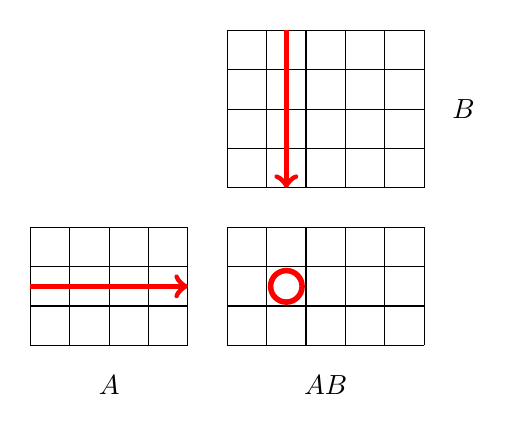
\begin{tikzpicture}[scale=0.5]
\draw (0,0) grid (4,3);
\draw (5,0) grid (10,3);
\draw (5,4) grid (10,8);

\node at (2,-1) {$A$};
\node at (7.5,-1) {$AB$};
\node at (11,6) {$B$};

\draw[thick,->,red,line width=2pt] (0,1.5) -- (4,1.5);
\draw[thick,->,red,line width=2pt] (6.5,8) -- (6.5,4);
\draw[thick,red,line width=2pt] (6.5,1.5) circle (0.4);
\end{tikzpicture}
\end{center}

\[
 \begin{bmatrix}
  1 & 4 \\
  3 & 9 \\
  8 & 6 \\
 \end{bmatrix}
\cdot
 \begin{bmatrix}
  1 & 6 \\
  2 & 9 \\
 \end{bmatrix}
=
 \begin{bmatrix}
  1 \cdot 1 + 4 \cdot 2 & 1 \cdot 6 + 4 \cdot 9 \\
  3 \cdot 1 + 9 \cdot 2 & 3 \cdot 6 + 9 \cdot 9 \\
  8 \cdot 1 + 6 \cdot 2 & 8 \cdot 6 + 6 \cdot 9 \\
 \end{bmatrix}
=
 \begin{bmatrix}
  9 & 42 \\
  21 & 99 \\
  20 & 102 \\
 \end{bmatrix}.
\]

行列の乗算において$A(BC)=(AB)C$は成立します。
ただし、可換ではないので、$AB=BA$は成立するとは限りません。

Matrix multiplication is associative,
so $A(BC)=(AB)C$ holds,
but it is not commutative,
so $AB = BA$ does not usually hold.

\index{単位行列 - identity matrix}

\key{単位行列 - identity matrix}とは、対角線上の各要素が1で、
それ以外の要素を0とする正方行列です。
例えば、次の行列は、$3 \times 3$の単位行列です

\[
 I = \begin{bmatrix}
  1 & 0 & 0 \\
  0 & 1 & 0 \\
  0 & 0 & 1 \\
 \end{bmatrix}
\]

\begin{samepage}
行列に単位行列をかけても行列は変わりません。
\[
 \begin{bmatrix}
  1 & 0 & 0 \\
  0 & 1 & 0 \\
  0 & 0 & 1 \\
 \end{bmatrix}
\cdot
 \begin{bmatrix}
  1 & 4 \\
  3 & 9 \\
  8 & 6 \\
 \end{bmatrix}
=
 \begin{bmatrix}
  1 & 4 \\
  3 & 9 \\
  8 & 6 \\
 \end{bmatrix} \hspace{10px} \textrm{and} \hspace{10px}
 \begin{bmatrix}
  1 & 4 \\
  3 & 9 \\
  8 & 6 \\
 \end{bmatrix}
\cdot
 \begin{bmatrix}
  1 & 0 \\
  0 & 1 \\
 \end{bmatrix}
=
 \begin{bmatrix}
  1 & 4 \\
  3 & 9 \\
  8 & 6 \\
 \end{bmatrix}.
\]
\end{samepage}

基本的なアルゴリズムを用いると、2つの$n \times n$の行列の積は$O(n^3)$ で計算できます。
行列の乗算にはより効率的なアルゴリズムがあります。しかし、それは数学的なものであり、競技プログラミングでは使われません。
\footnote{
最も最初のこの工夫は1969年に発表されたStrassenのアルゴリズム\cite{str69}で、
$O(n^{2.80735})$です。現在の最も優れたアルゴリズム \cite{gal14}は$O(n^{2.37286})$です。}

\subsubsection{行列の累乗 - Matrix power}

\index{行列の累乗 - matrix power}

$A^k$ は$A$が正方行列の時に定義されます。
これは次の様になります。
\[ A^k = \underbrace{A \cdot A \cdot A \cdots A}_{\textrm{$k$ times}} \]
例をあげます。

\[
 \begin{bmatrix}
  2 & 5 \\
  1 & 4 \\
 \end{bmatrix}^3 =
 \begin{bmatrix}
  2 & 5 \\
  1 & 4 \\
 \end{bmatrix} \cdot
 \begin{bmatrix}
  2 & 5 \\
  1 & 4 \\
 \end{bmatrix} \cdot
 \begin{bmatrix}
  2 & 5 \\
  1 & 4 \\
 \end{bmatrix} =
 \begin{bmatrix}
  48 & 165 \\
  33 & 114 \\
 \end{bmatrix}.
\]
また、$A^0$は単位行列とします。
\[
 \begin{bmatrix}
  2 & 5 \\
  1 & 4 \\
 \end{bmatrix}^0 =
 \begin{bmatrix}
  1 & 0 \\
  0 & 1 \\
 \end{bmatrix}.
\]

$A^k$ は21.2のアルゴリズムを使えば$O(n^3 \log k)$で求められます。
\[
 \begin{bmatrix}
  2 & 5 \\
  1 & 4 \\
 \end{bmatrix}^8 =
 \begin{bmatrix}
  2 & 5 \\
  1 & 4 \\
 \end{bmatrix}^4 \cdot
 \begin{bmatrix}
  2 & 5 \\
  1 & 4 \\
 \end{bmatrix}^4.
\]

\subsubsection{行列式 - Determinant}

\index{行列式 - determinant}

\key{行列式 - determinant}は、Aが正方行列である場合に定義されます。
Aが$1 \times 1$の大きさであれば、$\det(A)=A[1,1]$となります。
より大きな行列の行列式 は、次の式を用いて再帰的に計算されます
この時に\index{余因子 - cofactor}が用いられいます
\[\det(A)=\sum_{j=1}^n A[1,j] C[1,j],\]
$C[i,j]$は$A$における$[i,j]$の余因子で次の様に示されます。
\[C[i,j] = (-1)^{i+j} \det(M[i,j]),\]
$M[i,j]$は A から $i$ 行 $j$ 列を削除して得られる行列です。
係数$(-1)^{i+j}$により符号は毎回入れ替わります。
\[
\det(
 \begin{bmatrix}
  3 & 4 \\
  1 & 6 \\
 \end{bmatrix}
) = 3 \cdot 6 - 4 \cdot 1 = 14
\]
であり、
\[
\det(
 \begin{bmatrix}
  2 & 4 & 3 \\
  5 & 1 & 6 \\
  7 & 2 & 4 \\
 \end{bmatrix}
) =
2 \cdot
\det(
 \begin{bmatrix}
  1 & 6 \\
  2 & 4 \\
 \end{bmatrix}
)
-4 \cdot
\det(
 \begin{bmatrix}
  5 & 6 \\
  7 & 4 \\
 \end{bmatrix}
)
+3 \cdot
\det(
 \begin{bmatrix}
  5 & 1 \\
  7 & 2 \\
 \end{bmatrix}
) = 81.
\]

\index{逆行列 - inverse matrix}

The determinant of $A$ tells us
whether there is an \key{逆行列 - inverse matrix}
$A^{-1}$ such that $A \cdot A^{-1} = I$,
where $I$ is an identity matrix.
It turns out that $A^{-1}$ exists
exactly when $\det(A) \neq 0$,
and it can be calculated using the formula
$A$の行列式は、$A \cdot A^{-1} = I$($I$は単位行列)となる逆行列$A^{-1}$が存在するかどうかを教えてくれます。
$A^{-1}$は$\det(A) \neq 0$のときに正確に存在し、次式で計算できます。

\[A^{-1}[i,j] = \frac{C[j,i]}{det(A)}.\]

\[
\underbrace{
 \begin{bmatrix}
  2 & 4 & 3\\
  5 & 1 & 6\\
  7 & 2 & 4\\
 \end{bmatrix}
}_{A}
\cdot
\underbrace{
 \frac{1}{81}
 \begin{bmatrix}
   -8 & -10 & 21 \\
   22 & -13 & 3 \\
   3 & 24 & -18 \\
 \end{bmatrix}
}_{A^{-1}}
=
\underbrace{
 \begin{bmatrix}
  1 & 0 & 0 \\
  0 & 1 & 0 \\
  0 & 0 & 1 \\
 \end{bmatrix}
}_{I}.
\]

\section{線型回帰 - Linear recurrences}

\index{線形漸化式 - linear recurrence}

\key{線形漸化式 - linear recurrence}
は$f(n)$に対して$f(0),f(1),\ldots,f(k-1)$などの初期値が与えられている時に、
大きな$n$である
\[f(n) = c_1 f(n-1) + c_2 f(n-2) + \ldots + c_k f (n-k),\]
を求めたいとします。ここで $c_1,c_2,\ldots,c_k$ は定数です。

動的計画法では、$f(0),f(1),\ldots,f(n)$を順次計算することで、任意の$f(n)$を $O(kn)$で計算できる。
ですが、$k$ が小さい場合には行列演算を用いると、$O(k^3 \log n)$で求められ効率的なことがあります。

\subsubsection{フィボナッチ数 - Fibonacci numbers}

\index{フィボナッチ数 - Fibonacci number}

線形漸化式としてよくあるのはフィボナッチ数です。
\[
\begin{array}{lcl}
f(0) & = & 0 \\
f(1) & = & 1 \\
f(n) & = & f(n-1)+f(n-2) \\
\end{array}
\]
$k=2$ の時、 $c_1=c_2=1$です。

\begin{samepage}
フィボナッチ数の計算を効率的に行うために、
フィボナッチ式をサイズ$2 \times 2$の 正方行列$X$で表現すると、次のようになります。
\[ X \cdot
 \begin{bmatrix}
  f(i) \\
  f(i+1) \\
 \end{bmatrix}
=
 \begin{bmatrix}
  f(i+1) \\
  f(i+2) \\
 \end{bmatrix}
 \]
$f(i)$ と $f(i+1)$は
 $X$に対する''入力''で
$X$から$f(i+1)$ と $f(i+2)$
を求めていきます。

\[ X =
 \begin{bmatrix}
  0 & 1 \\
  1 & 1 \\
 \end{bmatrix}.
\]
\end{samepage}
\noindent
例としては、
\[
 \begin{bmatrix}
  0 & 1 \\
  1 & 1 \\
 \end{bmatrix}
\cdot
 \begin{bmatrix}
  f(5) \\
  f(6) \\
 \end{bmatrix}
=
 \begin{bmatrix}
  0 & 1 \\
  1 & 1 \\
 \end{bmatrix}
\cdot
 \begin{bmatrix}
  5 \\
  8 \\
 \end{bmatrix}
=
 \begin{bmatrix}
  8 \\
  13 \\
 \end{bmatrix}
=
 \begin{bmatrix}
  f(6) \\
  f(7) \\
 \end{bmatrix}.
\]
こうして$f(n)$を計算できます。
\[
 \begin{bmatrix}
  f(n) \\
  f(n+1) \\
 \end{bmatrix}
=
X^n \cdot
 \begin{bmatrix}
  f(0) \\
  f(1) \\
 \end{bmatrix}
=
 \begin{bmatrix}
  0 & 1 \\
  1 & 1 \\
 \end{bmatrix}^n
\cdot
 \begin{bmatrix}
  0 \\
  1 \\
 \end{bmatrix}.
\]
$X^n$ の値は $O(\log n)$  時間で計算できるため、$f(n)$ の値も $O(\log n)$  時間で計算できます。

\subsubsection{一般化 - General case}


では$f(n)$が任意の線形漸化式である一般的なケースを考えていきます。
目的は、以下のような行列 $X$ を構成することです。
\[ X \cdot
 \begin{bmatrix}
  f(i) \\
  f(i+1) \\
  \vdots \\
  f(i+k-1) \\
 \end{bmatrix}
=
 \begin{bmatrix}
  f(i+1) \\
  f(i+2) \\
  \vdots \\
  f(i+k) \\
 \end{bmatrix}.
\]
この様な行列は次の様になります。
\[
X =
 \begin{bmatrix}
  0 & 1 & 0 & 0 & \cdots & 0 \\
  0 & 0 & 1 & 0 & \cdots & 0 \\
  0 & 0 & 0 & 1 & \cdots & 0 \\
  \vdots & \vdots & \vdots & \vdots & \ddots & \vdots \\
  0 & 0 & 0 & 0 & \cdots & 1 \\
  c_k & c_{k-1} & c_{k-2} & c_{k-3} & \cdots & c_1 \\
 \end{bmatrix}.
\]
最初の$k - 1$行は、1つの要素が1であることを除いて、
各要素が0である。これらの 行は、$f (i)$ を$f (i + 1)$、$f (i + 1)$ を$f (i + 2)$、
と置き換えていきます。
最後の行には、 新しい値$f(i+k)$を計算するための漸化式の係数が含まれます。
\begin{samepage}
さて、$f (n)$ は次の式を用いて $O(k^3 \log n)$  時間で計算できます。
\[
 \begin{bmatrix}
  f(n) \\
  f(n+1) \\
  \vdots \\
  f(n+k-1) \\
 \end{bmatrix}
=
X^n \cdot
 \begin{bmatrix}
  f(0) \\
  f(1) \\
  \vdots \\
  f(k-1) \\
 \end{bmatrix}.
\]
\end{samepage}

\section{グラフと行列 - Graphs and matrices}

\subsubsection{パスのカウント - Counting paths}

グラフの隣接行列の累乗には、興味深い性質があります。
$V$が重みなしグラフの隣接行列であるとき、
行列 $V^n$ は、グラフのノード間の $n$ 本のエッジのパス の数を含んでいます。

\begin{center}
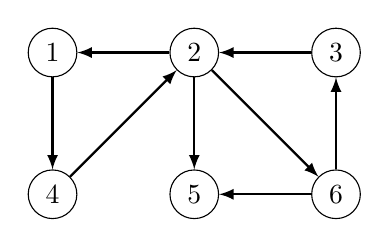
\begin{tikzpicture}[scale=0.9]
\node[draw, circle] (1) at (1,3) {$1$};
\node[draw, circle] (2) at (1,1) {$4$};
\node[draw, circle] (3) at (3,3) {$2$};
\node[draw, circle] (4) at (5,3) {$3$};
\node[draw, circle] (5) at (3,1) {$5$};
\node[draw, circle] (6) at (5,1) {$6$};

\path[draw,thick,->,>=latex] (1) -- (2);
\path[draw,thick,->,>=latex] (2) -- (3);
\path[draw,thick,->,>=latex] (3) -- (1);
\path[draw,thick,->,>=latex] (4) -- (3);
\path[draw,thick,->,>=latex] (3) -- (5);
\path[draw,thick,->,>=latex] (3) -- (6);
\path[draw,thick,->,>=latex] (6) -- (4);
\path[draw,thick,->,>=latex] (6) -- (5);
\end{tikzpicture}
\end{center}
この場合の隣接行列は、
\[
V= \begin{bmatrix}
  0 & 0 & 0 & 1 & 0 & 0 \\
  1 & 0 & 0 & 0 & 1 & 1 \\
  0 & 1 & 0 & 0 & 0 & 0 \\
  0 & 1 & 0 & 0 & 0 & 0 \\
  0 & 0 & 0 & 0 & 0 & 0 \\
  0 & 0 & 1 & 0 & 1 & 0 \\
 \end{bmatrix}.
\]
ここで、次を考えます。
\[
V^4= \begin{bmatrix}
  0 & 0 & 1 & 1 & 1 & 0 \\
  2 & 0 & 0 & 0 & 2 & 2 \\
  0 & 2 & 0 & 0 & 0 & 0 \\
  0 & 2 & 0 & 0 & 0 & 0 \\
  0 & 0 & 0 & 0 & 0 & 0 \\
  0 & 0 & 1 & 1 & 1 & 0 \\
 \end{bmatrix}
\]
contains the numbers of paths of 4 edges
between the nodes.
これは、パスが4のノードを示します。
例えば、$V^4[2,5]=2$ですが、
これはノード2とノード5の長さ4のパスは2つであることを示します。
$2 \rightarrow 1 \rightarrow 4 \rightarrow 2 \rightarrow 5$
と
$2 \rightarrow 6 \rightarrow 3 \rightarrow 2 \rightarrow 5$.
です。

\subsubsection{最短経路 - Shortest paths}

重み付きグラフも同様の考え方で、
ノードのペアごとに、
その間にちょうど $n$本のエッジを含むパスの最小の長さを計算することができます。
これを計算するためには、パスの数を計算するのではなくてパスの長さを最小にするように、
行列の乗算を新たに定義する必要があります。

\begin{samepage}
以下の例を考えます。
\begin{center}
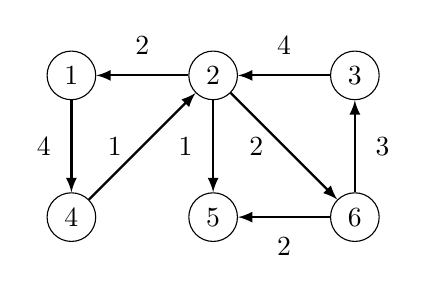
\begin{tikzpicture}[scale=0.9]
\node[draw, circle] (1) at (1,3) {$1$};
\node[draw, circle] (2) at (1,1) {$4$};
\node[draw, circle] (3) at (3,3) {$2$};
\node[draw, circle] (4) at (5,3) {$3$};
\node[draw, circle] (5) at (3,1) {$5$};
\node[draw, circle] (6) at (5,1) {$6$};

\path[draw,thick,->,>=latex] (1) -- node[font=\small,label=left:4] {} (2);
\path[draw,thick,->,>=latex] (2) -- node[font=\small,label=left:1] {} (3);
\path[draw,thick,->,>=latex] (3) -- node[font=\small,label=north:2] {} (1);
\path[draw,thick,->,>=latex] (4) -- node[font=\small,label=north:4] {} (3);
\path[draw,thick,->,>=latex] (3) -- node[font=\small,label=left:1] {} (5);
\path[draw,thick,->,>=latex] (3) -- node[font=\small,label=left:2] {} (6);
\path[draw,thick,->,>=latex] (6) -- node[font=\small,label=right:3] {} (4);
\path[draw,thick,->,>=latex] (6) -- node[font=\small,label=below:2] {} (5);
\end{tikzpicture}
\end{center}
\end{samepage}


$\infty$は辺が存在しないとし、各パスの重さを隣接グラフで表現します。

\[
V= \begin{bmatrix}
  \infty & \infty & \infty & 4 & \infty & \infty \\
  2 & \infty & \infty & \infty & 1 & 2 \\
  \infty & 4 & \infty & \infty & \infty & \infty \\
  \infty & 1 & \infty & \infty & \infty & \infty \\
  \infty & \infty & \infty & \infty & \infty & \infty \\
  \infty & \infty & 3 & \infty & 2 & \infty \\
 \end{bmatrix}.
\]

ここで、
\[
AB[i,j] = \sum_{k=1}^n A[i,k] \cdot B[k,j]
\]
という乗算を以下の様に定義します。
\[
AB[i,j] = \min_{k=1}^n A[i,k] + B[k,j]
\]

の代わりに最小値を、積の代わりに要素の和を計算します。
これだけで、行列の累乗はグラフの最短経路に対応します。

\[
V^4= \begin{bmatrix}
  \infty & \infty & 10 & 11 & 9 & \infty \\
  9 & \infty & \infty & \infty & 8 & 9 \\
  \infty & 11 & \infty & \infty & \infty & \infty \\
  \infty & 8 & \infty & \infty & \infty & \infty \\
  \infty & \infty & \infty & \infty & \infty & \infty \\
  \infty & \infty & 12 & 13 & 11 & \infty \\
 \end{bmatrix},
\]

ノード2からノード5までの4辺のパスの最小長は8です。
このようなパスは、
$2 \rightarrow 1 \rightarrow 4 \rightarrow 2 \rightarrow 5$.

\subsubsection{キルヒホッフの定理 - Kirchhoff's theorem}

\index{キルヒホッフの定理 - Kirchhoff's theorem}
\index{全域木 - spanning tree}

\key{キルヒホッフの定理 - Kirchhoff's theorem}
%\footnote{G. R. Kirchhoff (1824--1887) was a German physicist.}
グラフの全域木の数を特殊な行列の行列式として計算する方法です。

\begin{center}
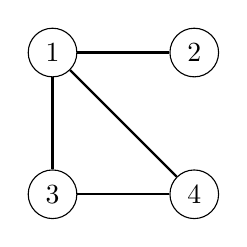
\begin{tikzpicture}[scale=0.9]
\node[draw, circle] (1) at (1,3) {$1$};
\node[draw, circle] (2) at (3,3) {$2$};
\node[draw, circle] (3) at (1,1) {$3$};
\node[draw, circle] (4) at (3,1) {$4$};

\path[draw,thick,-] (1) -- (2);
\path[draw,thick,-] (1) -- (3);
\path[draw,thick,-] (3) -- (4);
\path[draw,thick,-] (1) -- (4);
\end{tikzpicture}
\end{center}
これは3つの全域木があります。

\begin{center}
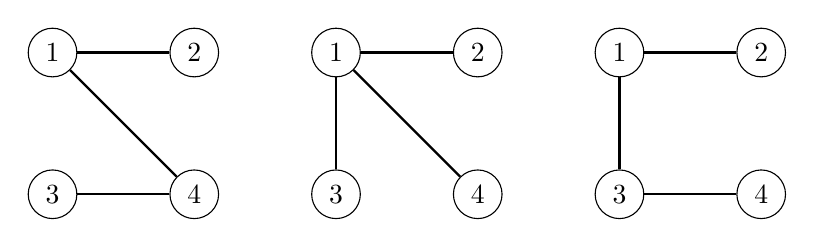
\begin{tikzpicture}[scale=0.9]
\node[draw, circle] (1a) at (1,3) {$1$};
\node[draw, circle] (2a) at (3,3) {$2$};
\node[draw, circle] (3a) at (1,1) {$3$};
\node[draw, circle] (4a) at (3,1) {$4$};

\path[draw,thick,-] (1a) -- (2a);
%\path[draw,thick,-] (1a) -- (3a);
\path[draw,thick,-] (3a) -- (4a);
\path[draw,thick,-] (1a) -- (4a);

\node[draw, circle] (1b) at (1+4,3) {$1$};
\node[draw, circle] (2b) at (3+4,3) {$2$};
\node[draw, circle] (3b) at (1+4,1) {$3$};
\node[draw, circle] (4b) at (3+4,1) {$4$};

\path[draw,thick,-] (1b) -- (2b);
\path[draw,thick,-] (1b) -- (3b);
%\path[draw,thick,-] (3b) -- (4b);
\path[draw,thick,-] (1b) -- (4b);

\node[draw, circle] (1c) at (1+8,3) {$1$};
\node[draw, circle] (2c) at (3+8,3) {$2$};
\node[draw, circle] (3c) at (1+8,1) {$3$};
\node[draw, circle] (4c) at (3+8,1) {$4$};

\path[draw,thick,-] (1c) -- (2c);
\path[draw,thick,-] (1c) -- (3c);
\path[draw,thick,-] (3c) -- (4c);
%\path[draw,thick,-] (1c) -- (4c);
\end{tikzpicture}
\end{center}
\index{Laplacean matrix}
全域木の数を計算するために、
$L[i, i]$ をノード $i$ の次数とし、ノード $i$ と $j$ の間にエッジがあれば
$L[i, j] = -1$、なければ $L[i, j] = 0$ の\key{ラプラシアン行列 - Laplacean matrix} を構成します。
上記のグラフのラプラシアン行列は次の様になります。

\[
L= \begin{bmatrix}
  3 & -1 & -1 & -1 \\
  -1 & 1 & 0 & 0 \\
  -1 & 0 & 2 & -1 \\
  -1 & 0 & -1 & 2 \\
 \end{bmatrix}
\]

全域木の数は、$L$から任意の行と列を削除したときに得られる行列の行列式に等しいです。

\[ \det(
\begin{bmatrix}
  1 & 0 & 0 \\
  0 & 2 & -1 \\
  0 & -1 & 2 \\
 \end{bmatrix}
) =3.\]

$L$からどの行と列を削除しても、行列式は常に同じです。

なお、22.5章のCayleyの公式はKirchhoffの定理の特殊な例で、ノード数$n$の完全グラフです。

\[ \det(
\begin{bmatrix}
  n-1 & -1 & \cdots & -1 \\
  -1 & n-1 & \cdots & -1 \\
  \vdots & \vdots & \ddots & \vdots \\
  -1 & -1 & \cdots & n-1 \\
 \end{bmatrix}
) =n^{n-2}.\]
